\documentclass[a4paper,10pt]{report}
\usepackage[utf8]{inputenc}
\usepackage{graphicx}
\usepackage{subcaption}
\usepackage{wrapfig}
\newcommand{\comments}[1]{}

% Title Page
\title{Implémentation d'article de recherche \\ 
Removing Camera Shake via Weighted Fourier Burst Accumulation}
\author{Sofiane Horache, Roman Fenioux}
\date{April 2017}


\begin{document}
\maketitle

% pour éviter d'avoir la numérotation 0.1 0.2 etc avant les sections
\setcounter{secnumdepth}{0}

% 1st page, résumé de l'article
\section{Introduction}
\paragraph{}
Le problème adressé ici est le flou de bougé, présent notamment dans les photographies 
amateur prises à la main dans des environnements mal éclairés. Pour avoir une photographie 
suffisament exposée il est souvent necessaire d'augmenter le temps d'exposition lorsqu'on 
ne peut ou ne veut pas agir sur l'ouverture ou la sensibilité de l'appareil. Mais si la 
position de l'appareil change durant l'acquisition, on voit apparaître du flou dans la direction
du mouvement. 

\section{Approche de l'article}
\paragraph{}
Le mouvement de l'appareil durant la prise de vue peut-être modélisé par une convolution de l'image
par un noyau de flou. la direction du mouvement est aléatoire d'une image à l'autre et on veut donc 
récupérer l'information que contient chaque image pour obtenir une image nette. L'approche utilisée 
ici consiste à prendre une rafale d'images au lieu d'une seule, puis à les combiner pour éliminer ce 
flou. Cette technique permet même de débruiter l'image. Pour une séquence de M images on a :
\[
  v_{i} = u_{i} \ast k_{i} + n{i}
\]
Pour ce faire l'article propose de calculer une moyenne pondérée de leurs transformées 
de Fourier pour éviter d'avoir à faire une estimation explicite du noyau de flou.
\[
  u_{p}(x) = \mathcal{F}^{-1}\left(\sum_{i=1}^M w_{i}(\zeta)\cdot \hat{v_{i}}(\zeta)\right)(x)
\]
\[
  w_{i}(\zeta) = \frac{|\hat{v_{i}}(\zeta)|^p}{\sum_{j=1}^M |\hat{v_{j}}(\zeta)|^p}
\]

\section{Notre implémentation}
\paragraph{}
A compléter : explications sur ce qu'on a fait
\paragraph{}
Nous avons d'abord implémenté la méthode de l'article sur des images supposées bien recalées, puis
nous avons implémenté l'algorithme ORSA pour le recalage des images. 
Nous n'avons pas implémenté la détection des homographies dégénérées.

\section{Nos résultats}
\paragraph{}
A compléter : illustrations de nos tests et résultats\\
Tests: robustesse bruit, robustesse grand mouvements, test différents p
\subsection{Images déjà recalées}
Nous avons d'abord testé la méthode sur des images déjà recalées : 
les images anthropologies utilisées dans l'articles ainsi que d'autres que nous avons faites 
nous même avec des noyaus de flous correspondant à un mouvement linéaire. Dans la figure~\ref{fig:arctriomphe}
page~\pageref{fig:arctriomphe} on peut comparer le résultat obtenu à
l'image originale utilisée et à la meilleure des images floues.

\begin{figure}[h]
 
\begin{subfigure}{0.24\textwidth}
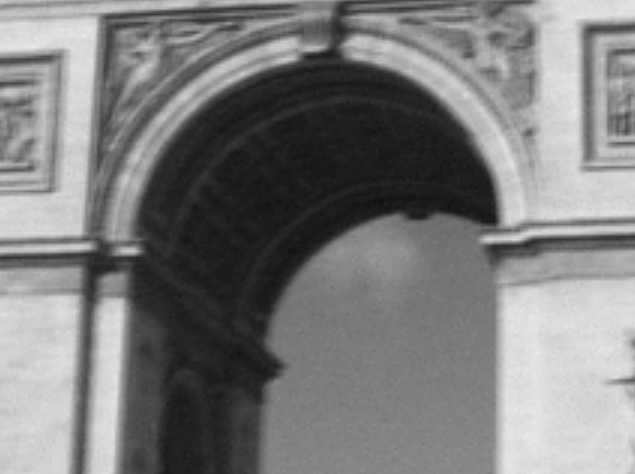
\includegraphics[width=0.9\linewidth, height=2.5cm]{ressource/detail_flou1.png} 
\caption{Input 1}
\label{fig:Flou1}
\end{subfigure}
\begin{subfigure}{0.24\textwidth}
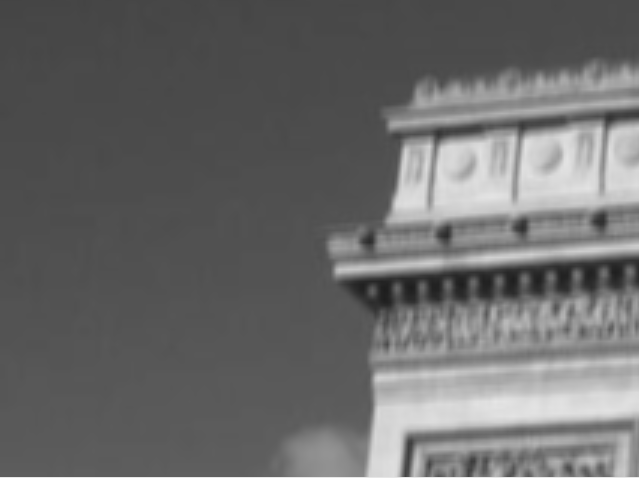
\includegraphics[width=0.9\linewidth, height=2.5cm]{ressource/detail_flou2.png}
\caption{Input 2}
\label{fig:Flou2}
\end{subfigure}
\begin{subfigure}{0.24\textwidth}
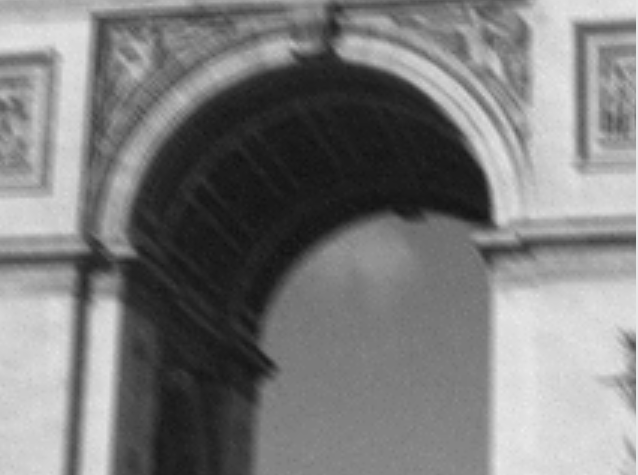
\includegraphics[width=0.9\linewidth, height=2.5cm]{ressource/detail_flou3.png}
\caption{Input 3}
\label{fig:Flou3}
\end{subfigure}
\begin{subfigure}{0.24\textwidth}
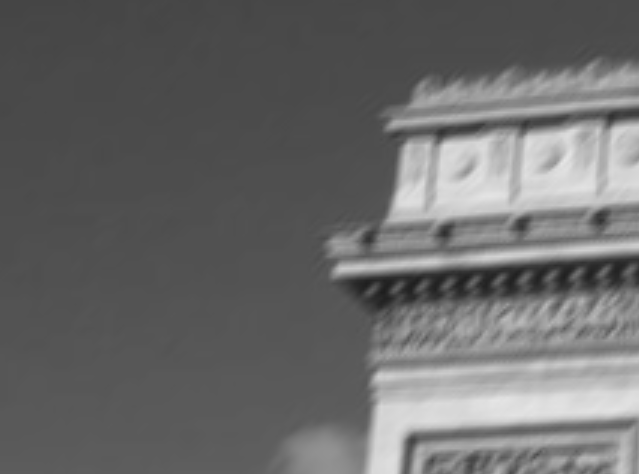
\includegraphics[width=0.9\linewidth, height=2.5cm]{ressource/detail_flou4.png}
\caption{Input 4}
\label{fig:Flou4}
\end{subfigure}
\begin{subfigure}{0.32\textwidth}
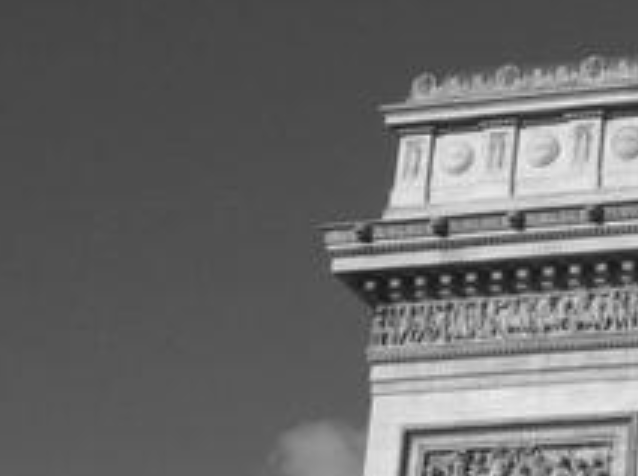
\includegraphics[width=0.9\linewidth, height=3.3cm]{ressource/detail_orig.png}
\caption{Original sans flou}
\label{fig:Original}
\end{subfigure}
\begin{subfigure}{0.32\textwidth}
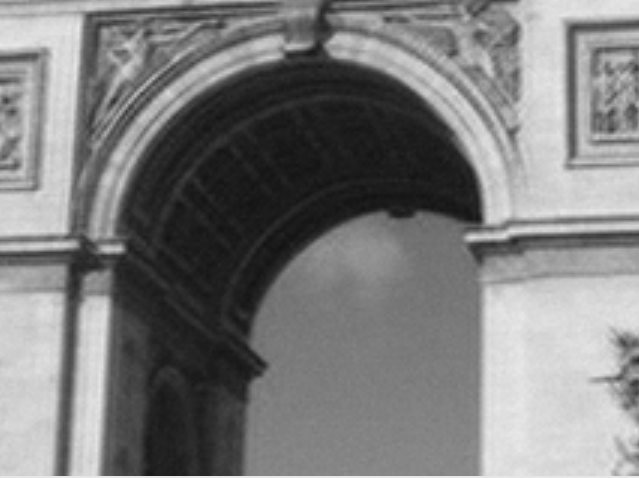
\includegraphics[width=0.9\linewidth, height=3.3cm]{ressource/detail_result.png}
\caption{Résultat}
\label{fig:Resultat}
\end{subfigure}
\begin{subfigure}{0.32\textwidth}
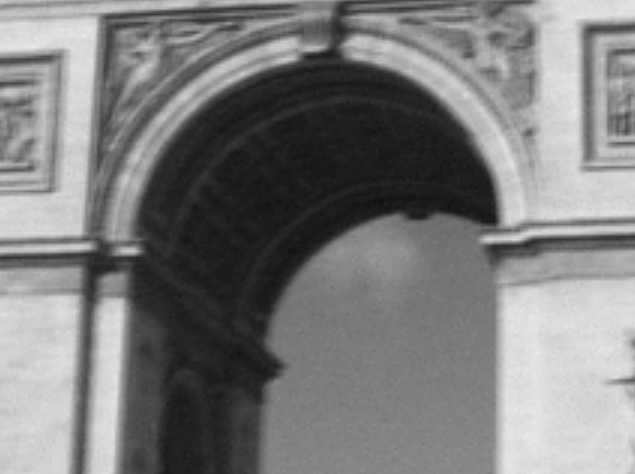
\includegraphics[width=0.9\linewidth, height=3.3cm]{ressource/detail_flou1.png} 
\caption{Meilleur input}
\label{fig:Bestflou}
\end{subfigure}

\caption{Résultat de l'algorithme pour 4 images recalées}
\label{fig:arctriomphe}
\end{figure}

\subsection{Images non recalées}
\paragraph{}
Dans la phase de recalage, le nombre d'iteration utilisé joue un rôle très important. 
\\\\
INSERER IMAGE AVEC 1000 iter vs 2000 iter (vs 10000 iter)



\section{Analyse et Commentaires}
\paragraph{}
A compléter : analyse de la méthode, points forts / faibles, limites et améliorations possibles
Pb : recalage d'images floues.. ? tester les limites

\subsection{Recalage des images}

\paragraph{}
Le recalage s'avère être le point critique de notre implémentation. 
Une erreur lors du recalage d'une seule des images 
engendre de très gros défauts dans le résultat comme on le voit sur la 
figure~\ref{fig:mauvaisrecalage} page~\pageref{fig:mauvaisrecalage}.
Ce problème nous a conduit à rejeter les images dont l'estimation d'homographie
s'appuie sur un nombre de points trop faibles. Nous utilisons donc ici le critère : 
image rejetée si \(n_{inliers} < 100\). 
Nous sommes bien sûr conscient qu'un meilleur critère devrait être utilisé. 

\begin{figure}[h]
\centering
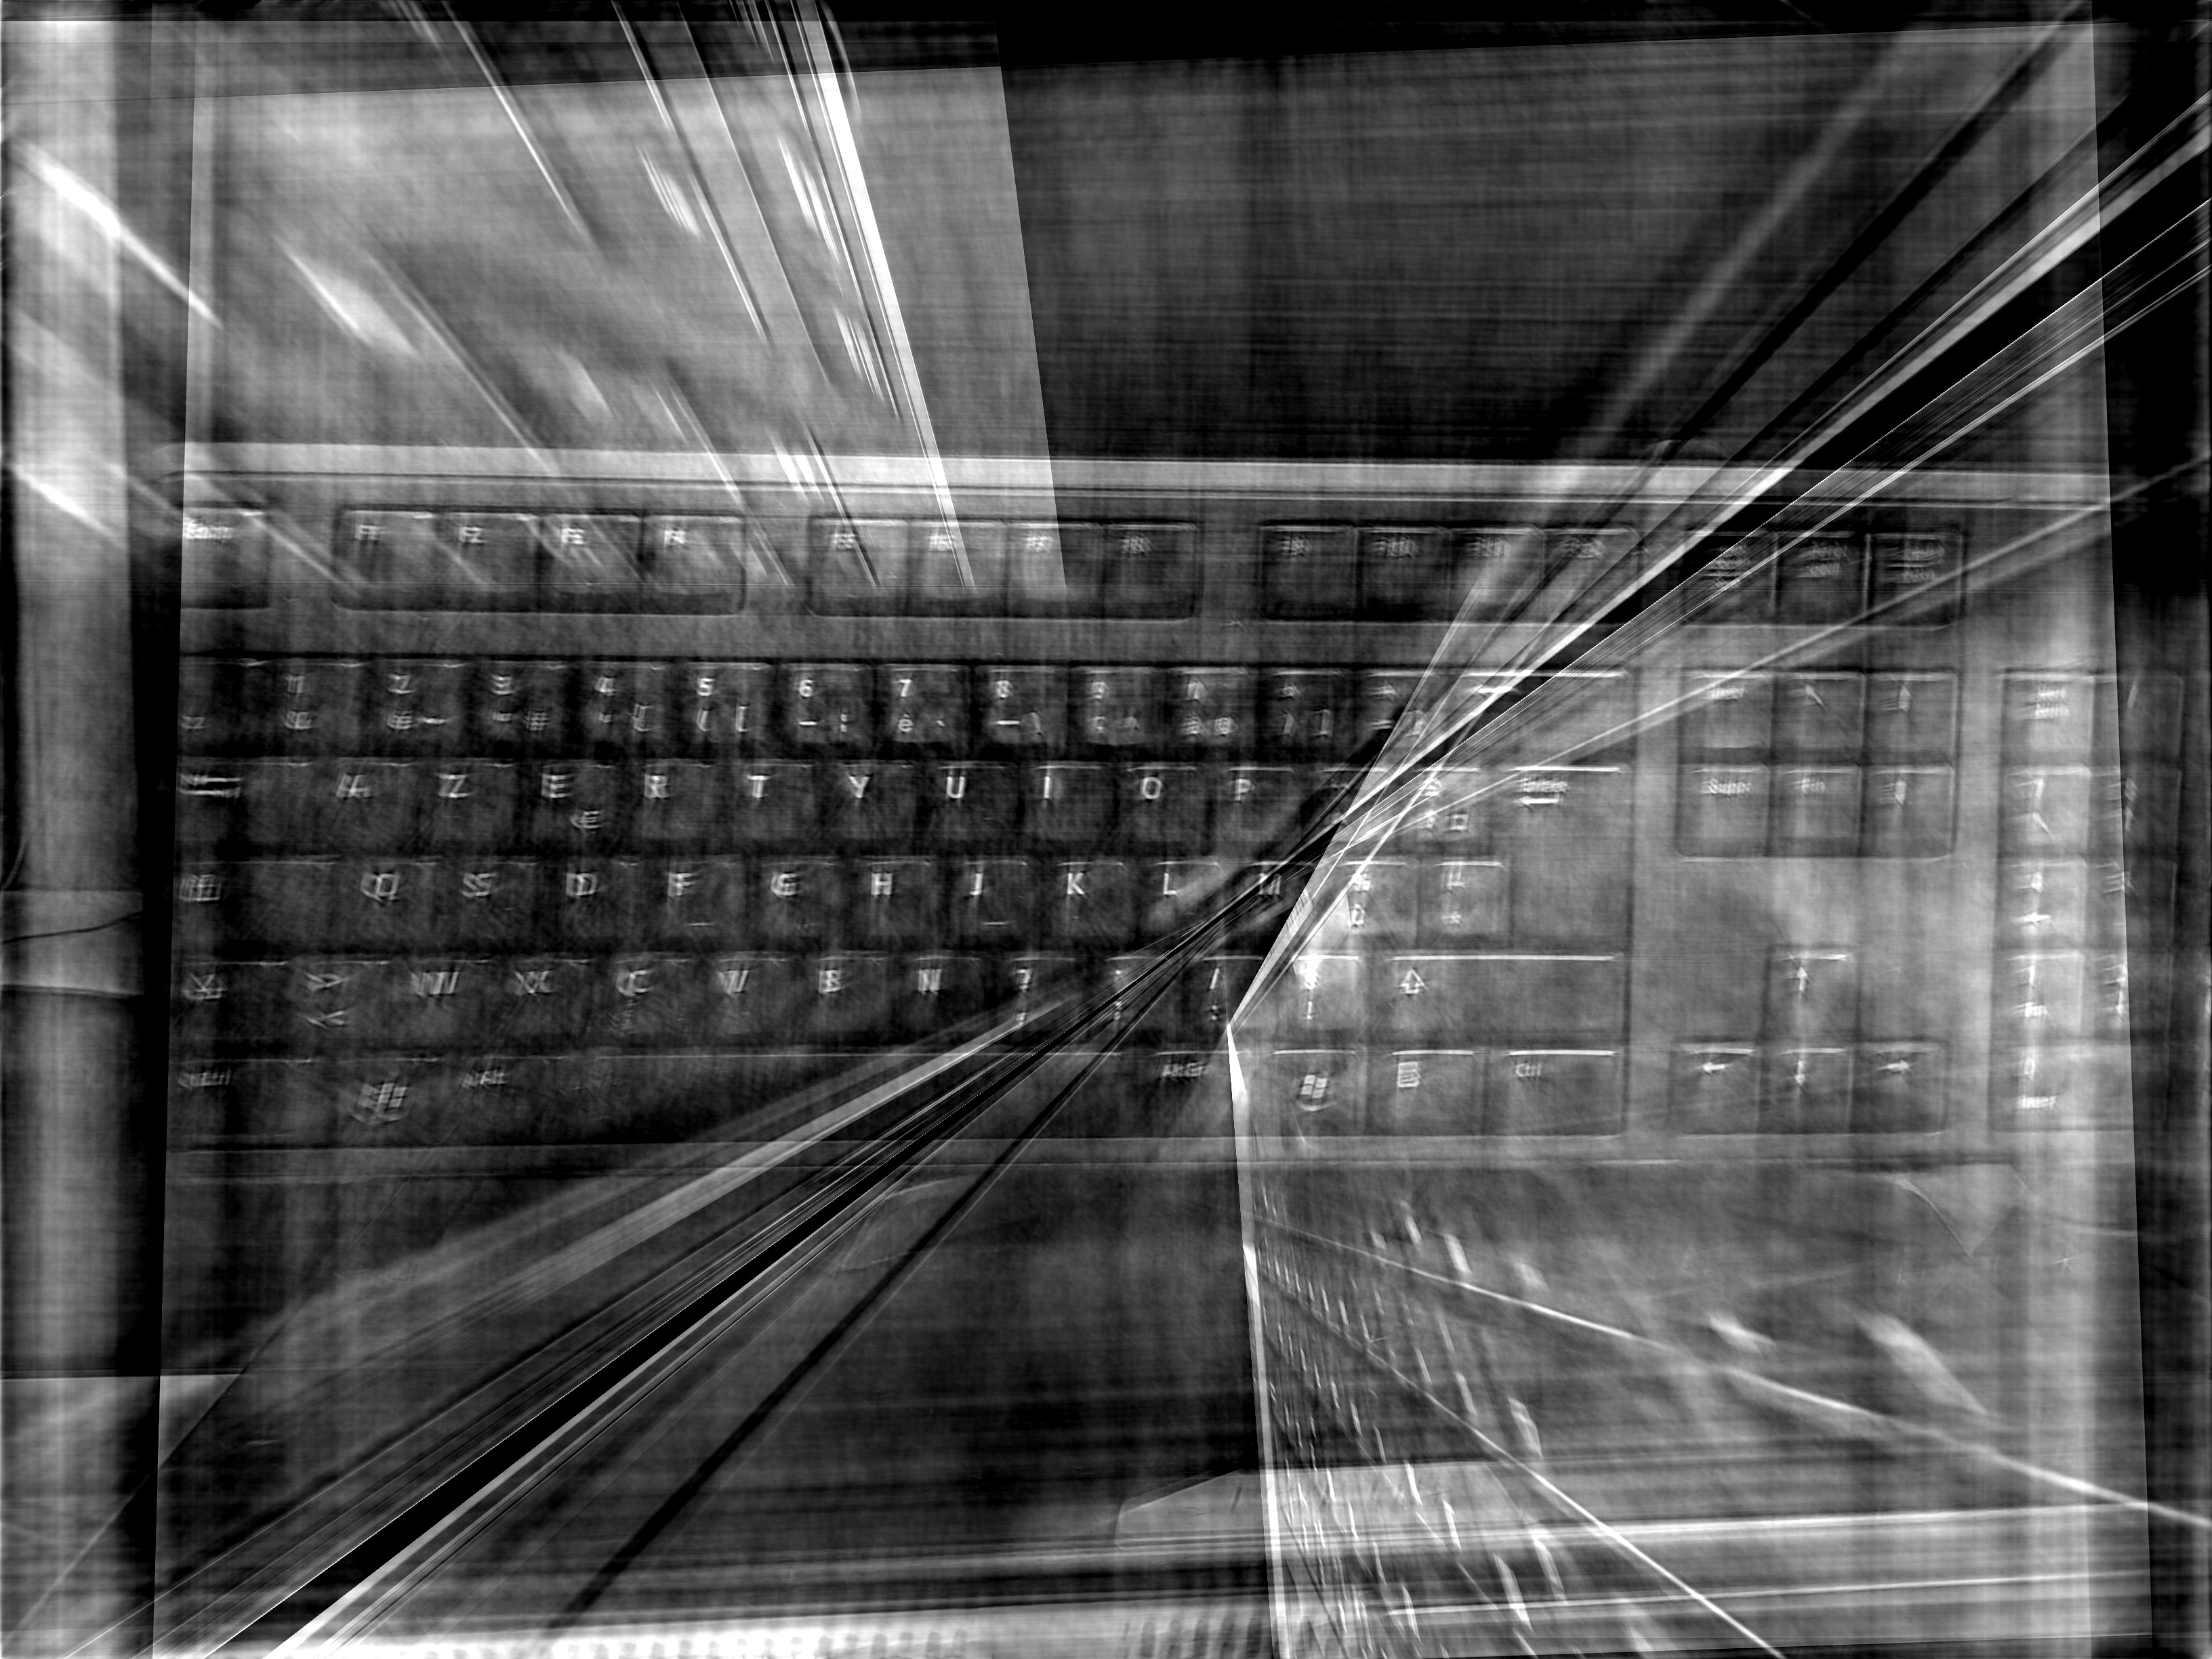
\includegraphics[width=0.5\linewidth]{ressource/keyboardresultat.jpg} 
\caption{Resultat suite à un mauvais recalage}
\label{fig:mauvaisrecalage}
\end{figure}


\subsection{Compromis temps de calcul - précision}
\paragraph{}
La phase de recalage peux prendre beaucoup de temps, mais est extrêmement importante pour avoir de bons résultats.
Sur nos exemples il est nécessaire d'avoir au moins 2000 iterations dans l'algorithme ORSA pour obtenir un 
recalage satisfaisant. 
L'article évite cette question en supposant que le recalage est fait immédiatement grâce aux gyroscopes
des smartphones, mais cela peut constituer une limite à l'application de la méthode en temps réel dans 
d'autres appareils. Cependant on peut imaginer que se problème se règle avec l'augmentation des capacité de calcul 
des appareils.

\subsection{Flou non homogène : mouvement rotatif}
\paragraph{}
Une limite intrinsèque à cette méthode est l'hypothèse que le flou peut être modélisé comme une convolution
par un noyau. C'est le cas pour les mouvement de translation et de certaines rotations mais ce n'est plus possible 
lorsque l'appareil subit une rotation autour de son axe optique. La PSF dépend alors de la position du pixel dans l'image, 
ce qui ne peut pas être modélisé par une convolution avec un noyau.
\paragraph{}
Ce cas de figure peut pourtant se produire en situation réelle comme nous l'avons constaté 
(Figure~\ref{fig:rotation} page~\pageref{fig:rotation})

\begin{figure}[h]

\begin{subfigure}{0.32\textwidth}
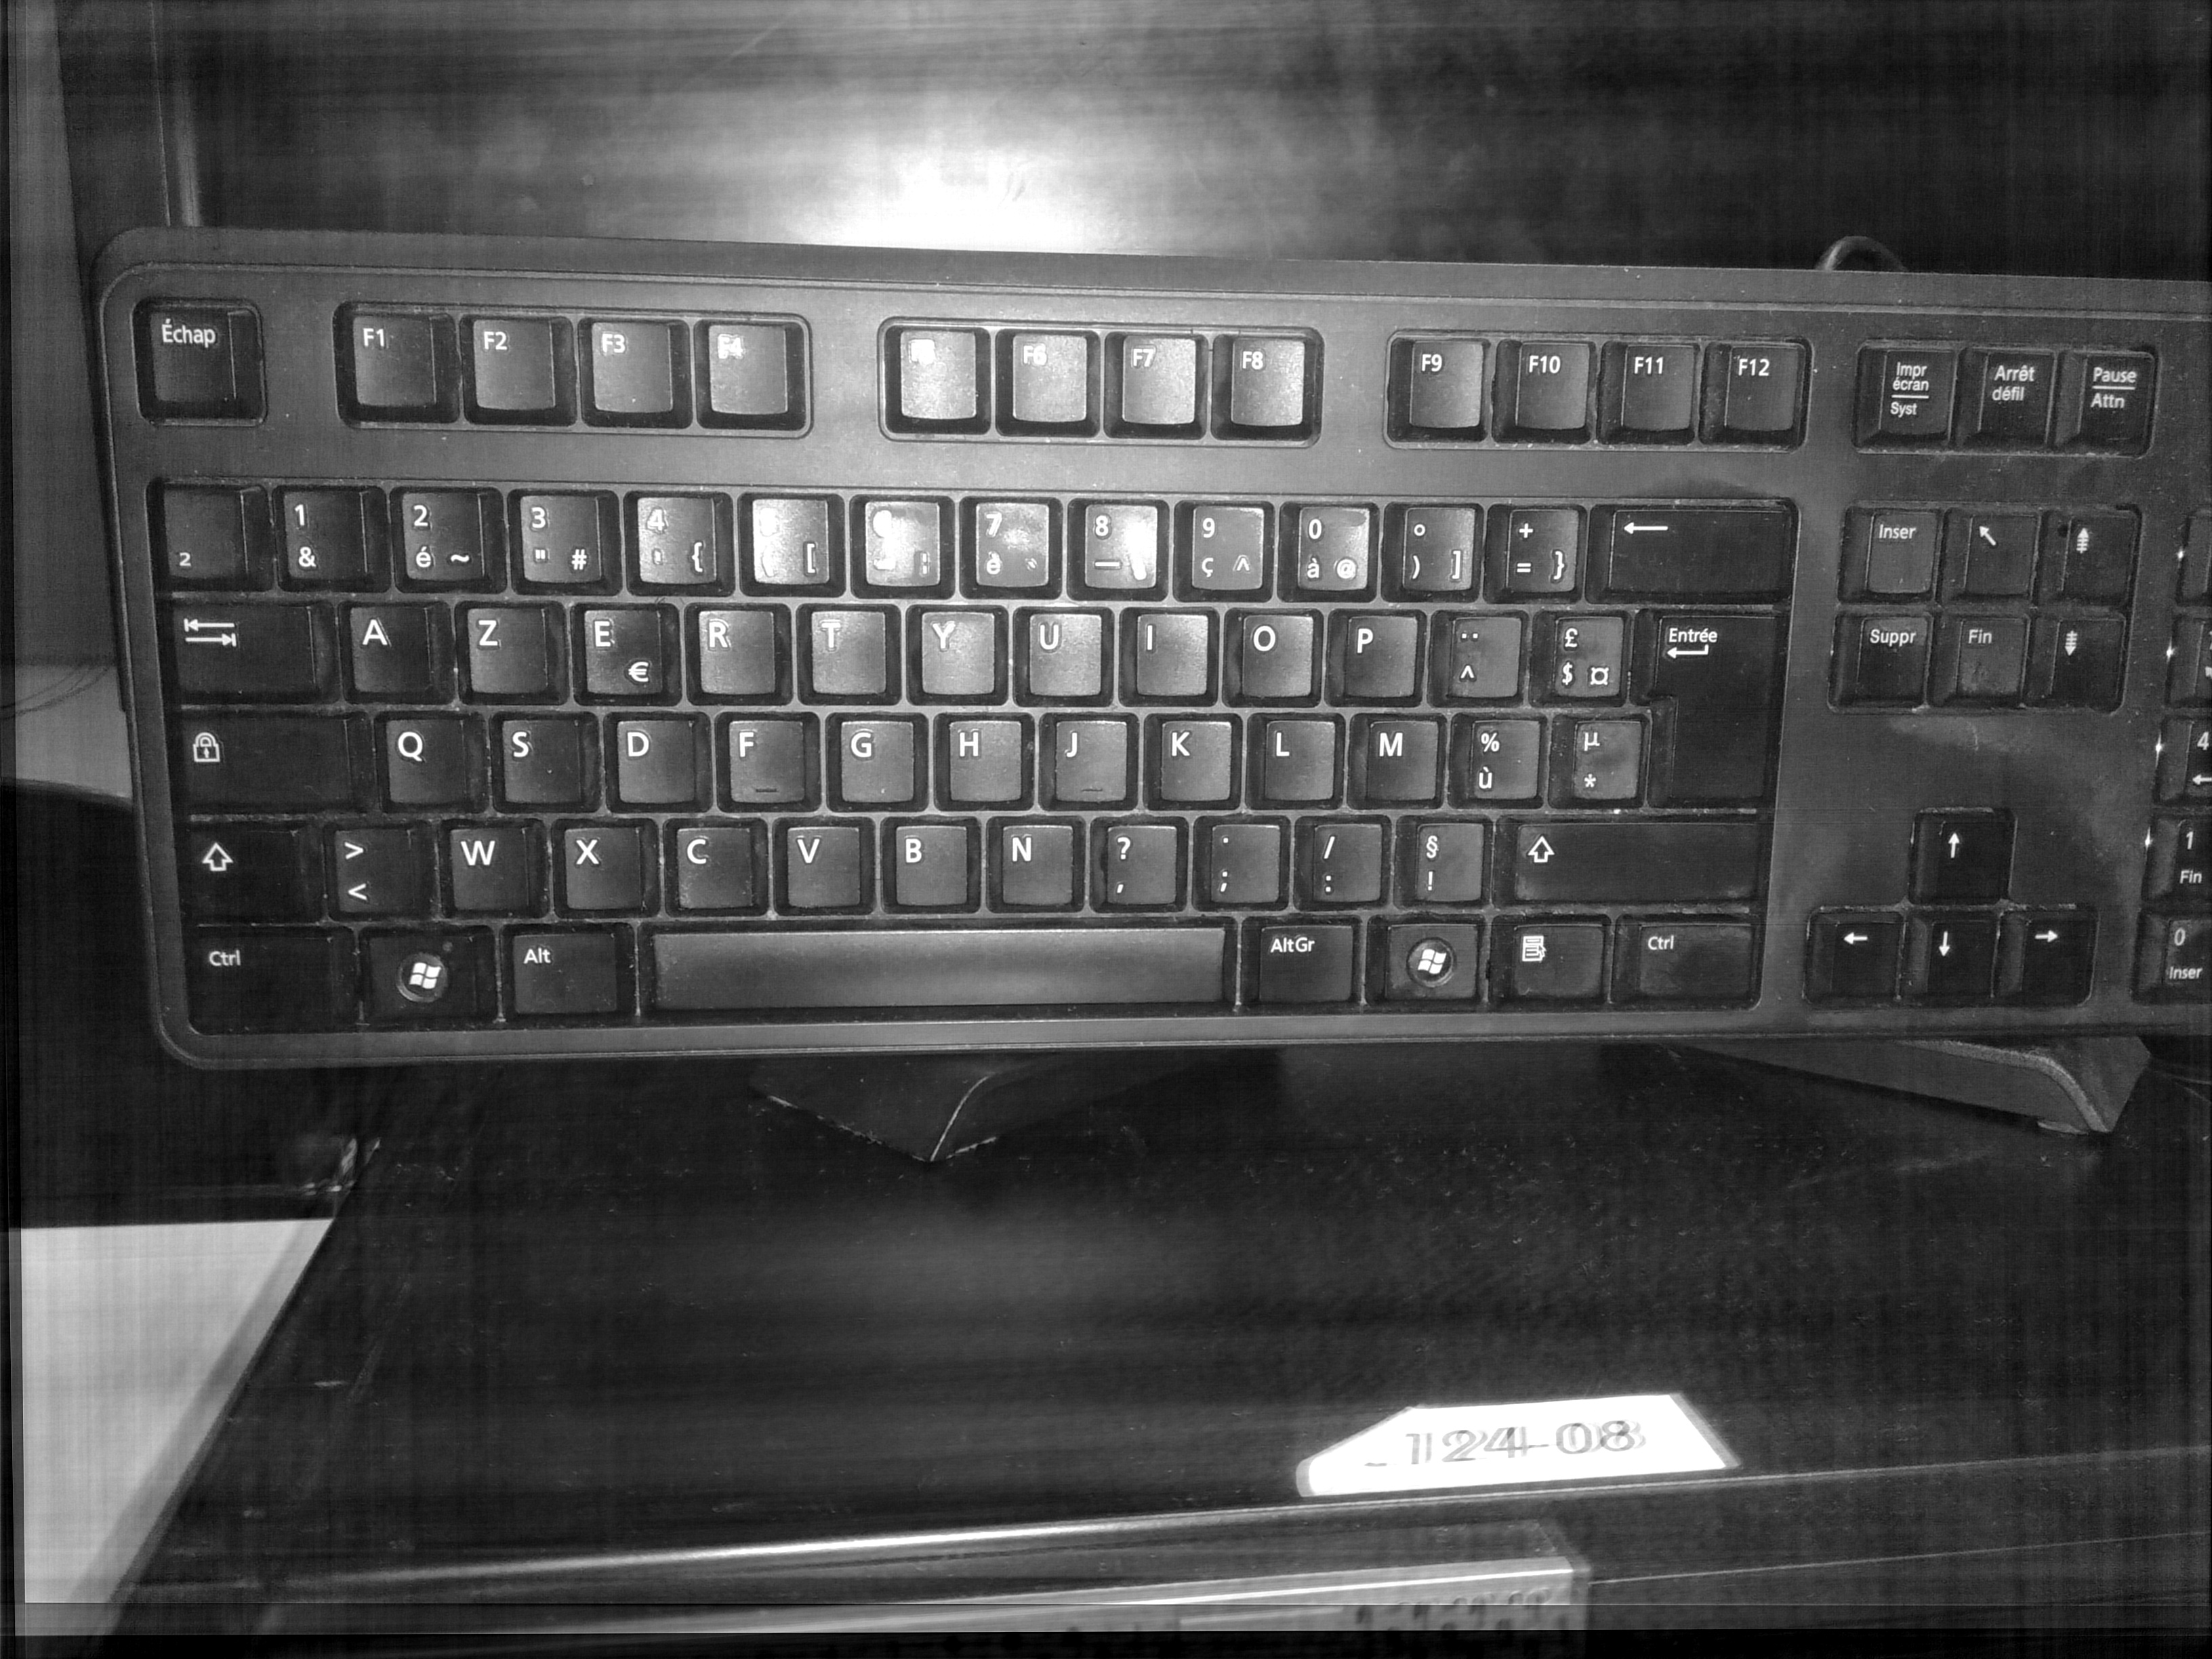
\includegraphics[width=0.9\linewidth]{ressource/flou_rot_10kit.jpg} 
\caption{Resultat}
\label{fig:Bestflou}
\end{subfigure}
\begin{subfigure}{0.32\textwidth}
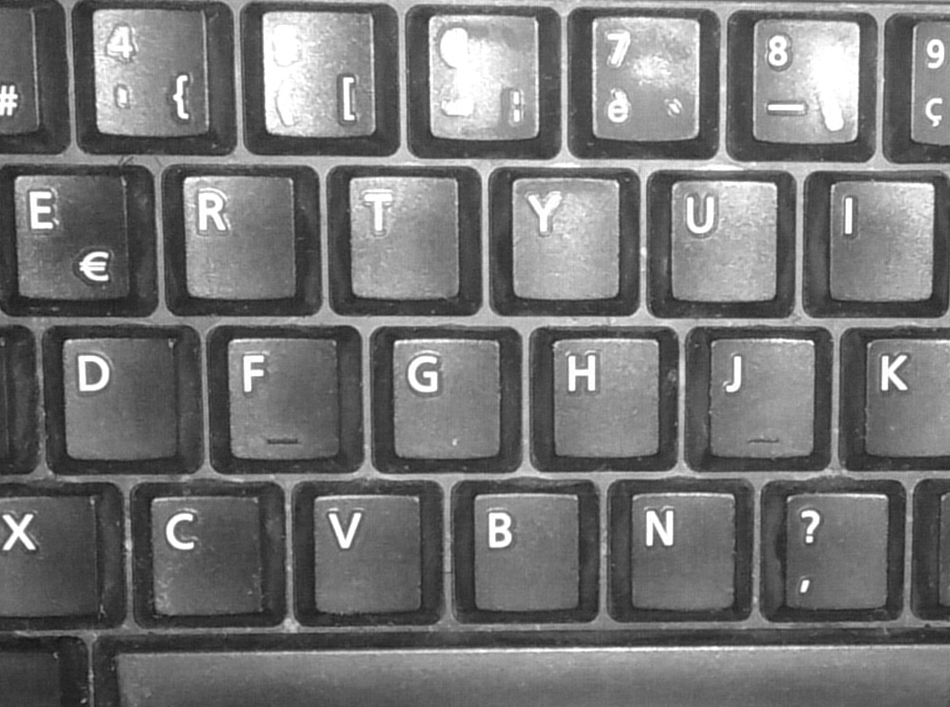
\includegraphics[width=0.9\linewidth]{ressource/flou_rot_centre.png} 
\caption{Centre de l'image}
\label{fig:flouRotCenter}
\end{subfigure}
\begin{subfigure}{0.32\textwidth}
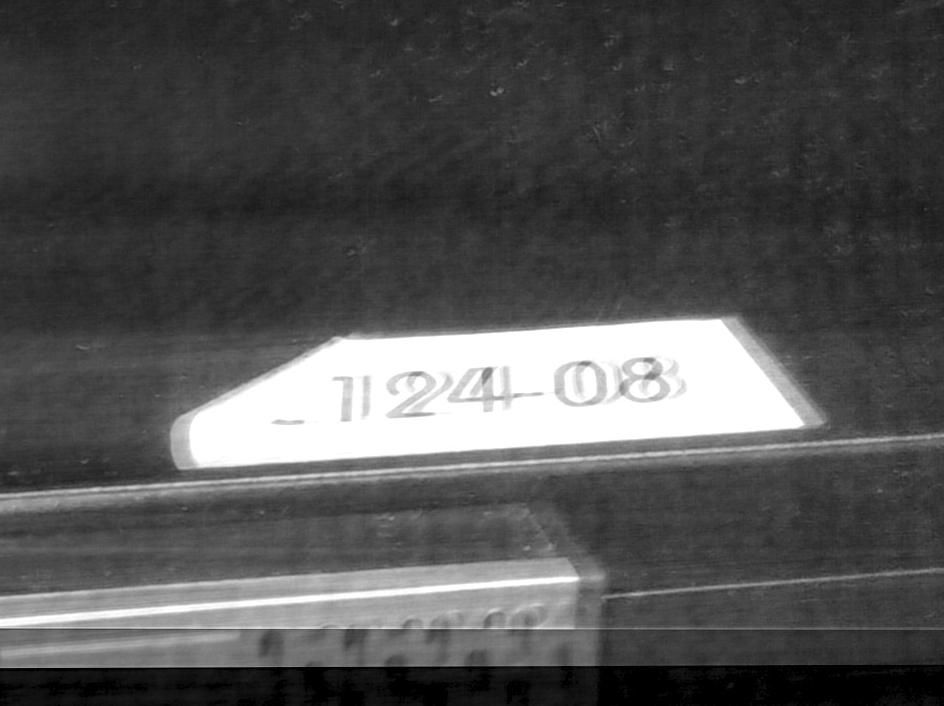
\includegraphics[width=0.9\linewidth]{ressource/flou_rot_bottom.png} 
\caption{Bas de l'image}
\label{fig:flouRotBottom}
\end{subfigure}


\caption{Resultat suite à un mauvais recalage}
\label{fig:rotation}
\end{figure}

\paragraph{}
Le résultat est très bon au centre de l'image mais se dégrade vers les bords. Une solution envisageable pourrait être
d'appliquer l'algorithme localement sur des portions de l'image suffisamment petite pour que 
l'hypothèse de convolution par un noyau de flou soit valable.

\end{document}          
